\documentclass[aspectratio=169]{beamer}

\usepackage[utf8]{inputenc}
\usepackage{amsmath}
\usepackage{amsfonts}
\usepackage{amssymb}
\usepackage{graphicx}
\usepackage{ragged2e}
\usepackage{booktabs}
\usepackage{tabularx}
\usepackage{tikz}
\usetikzlibrary{calc, shapes, backgrounds}
\usepackage{amsmath}
\usepackage{amssymb}
\usepackage{dsfont}
\usepackage{url}
\usepackage{listings}
\usepackage[T1]{fontenc}

\usepackage{theme/beamerthemehbrs}

\author[Ujjwal]{Ujjwal Patil}
\title{Introduction to Linux}
\subtitle{Foundation Course -- Winter Semester 2026}
\institute[HBRS]{Hochschule Bonn-Rhein-Sieg}
\date{September 10, 2026}
\subject{Linux}

\def\advisors{}
% \thirdpartylogo{path/to/logo}
\AtBeginSection{}
\begin{document}

{
\begin{frame}
\titlepage
\end{frame}
}

% Tell LaTeX where to find images, and set code font size globally
\graphicspath{{images/}}
\lstset{basicstyle=\ttfamily\footnotesize, tabsize=2, breaklines=true, breakatwhitespace=true}

% ====================================================================
\section{What is GNU/Linux?}
% ====================================================================

\begin{frame}{What is GNU/Linux?}
  \begin{columns}
    \column{.6\textwidth}
      \begin{itemize}
        \item \alert{Free}, open-source, Unix-like operating system
        \item \alert{Kernel} written by Linus Torvalds in 1991
        \item GNU tools + Linux kernel = \alert{GNU/Linux}
        \item Many \alert{distributions} (distros) available:\\
              Ubuntu, Fedora, Debian, Arch, openSUSE \ldots
      \end{itemize}
      \vspace{0.4em}
      \begin{exampleblock}{This course}
        Ubuntu 22.04 LTS (Jammy Jellyfish)
      \end{exampleblock}      
    \column{.4\textwidth}
      \begin{center}
        
\includegraphics[width=\columnwidth, height=0.72\textheight, keepaspectratio]
          {tux_and_distros.png}
      \end{center}
  \end{columns}
  \begin{alertblock}{Why Linux for robotics?}
        ROS2 Humble is only officially supported on Ubuntu 22.04.
        Every robot you will program here runs Linux.
      \end{alertblock}
\end{frame}

\begin{frame}{Linux is Everywhere}
  \framesubtitle{You already use it every day}
  \begin{columns}
    \column{.5\textwidth}
      \begin{itemize}
        \item \textbf{Android} -- every phone in your pocket
        \item \textbf{Servers} -- powers most of the internet
        \item \textbf{Supercomputers} -- 100\% of TOP500
        \item \textbf{Smart TVs, routers, embedded systems}
        \item \textbf{Robotics} -- ROS2 runs natively on Linux
      \end{itemize}
      \vspace{0.4em}
      \begin{block}{The GNU/Linux stack}
        Hardware $\rightarrow$ Kernel $\rightarrow$ GNU Tools
        $\rightarrow$ Shell $\rightarrow$ Applications
      \end{block}
    \column{.5\textwidth}
      \begin{alertblock}{Why it matters here}
        Learning the terminal is not optional.
        It is the primary interface for ROS2,
        robotics, and remote systems over SSH.
      \end{alertblock}
  \end{columns}
\end{frame}

\begin{frame}{Linux Directory Tree}
  \framesubtitle{No drive letters -- one single tree starting at / (root)}
  \begin{columns}
    \column{.44\textwidth}
      \begin{itemize}
        \item Root is \alert{\texttt{/}} -- top of the tree
        \item System folders: \textbf{protected} (need \texttt{sudo})
        \item \alert{Your space}: \texttt{/home/username}
        \item \alert{\texttt{\textasciitilde}} always means your home
      \end{itemize}
      \vspace{0.4em}
      \begin{block}{Key system folders}
        \texttt{/bin} \quad essential programs\\
        \texttt{/usr} \quad installed software\\
        \texttt{/etc} \quad configuration files\\
        \texttt{/tmp} \quad temporary files
      \end{block}
    \column{.56\textwidth}
      \begin{center}
        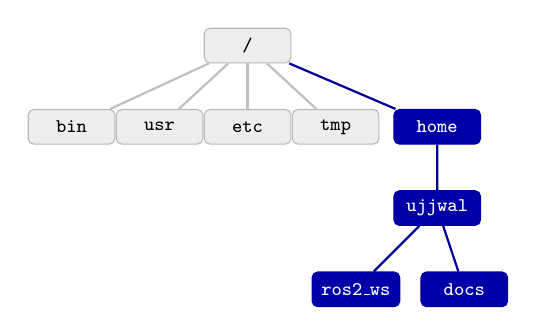
\begin{tikzpicture}[
          scale=0.86,
          sys/.style={rectangle, rounded corners=2pt, draw=gray!55,
                      fill=gray!14, minimum width=1.10cm,
                      minimum height=0.44cm, text centered,
                      font=\ttfamily\scriptsize},
          own/.style={rectangle, rounded corners=2pt,
                      draw=blue!65!black, fill=blue!65!black,
                      text=white, minimum width=1.10cm,
                      minimum height=0.44cm, text centered,
                      font=\ttfamily\scriptsize\bfseries}
        ]
          \node[sys] (root) at (0,0)       {/};
          \node[sys] (bin)  at (-2.6,-1.2) {bin};
          \node[sys] (usr)  at (-1.3,-1.2) {usr};
          \node[sys] (etc)  at  (0.0,-1.2) {etc};
          \node[sys] (tmp)  at  (1.3,-1.2) {tmp};
          \node[own] (home) at  (2.8,-1.2) {home};
          \node[own] (me)   at  (2.8,-2.4) {ujjwal};
          \node[own] (ws)   at  (1.6,-3.6) {ros2\_ws};
          \node[own] (doc)  at  (3.2,-3.6) {docs};
          \draw[gray!50, thick] (root)--(bin);
          \draw[gray!50, thick] (root)--(usr);
          \draw[gray!50, thick] (root)--(etc);
          \draw[gray!50, thick] (root)--(tmp);
          \draw[blue!58!black, thick] (root)--(home);
          \draw[blue!58!black, thick] (home)--(me);
          \draw[blue!58!black, thick] (me)--(ws);
          \draw[blue!58!black, thick] (me)--(doc);
        \end{tikzpicture}\\[0.2em]
        {\tiny \alert{Blue} = your space. \quad Gray = system (protected).}
      \end{center}
  \end{columns}
\end{frame}

\begin{frame}{Files and Folders}
  \begin{columns}
    \column{.5\textwidth}
      \begin{block}{Folders end with /}
        \texttt{/home/ujjwal/projects/}
      \end{block}
      \vspace{0.35em}
      \begin{block}{Everything else is a file}
        \texttt{/home/ujjwal/main.cpp}
      \end{block}
      \vspace{0.35em}
      \begin{alertblock}{Paths are case sensitive!}
        \texttt{main.cpp} $\neq$ \texttt{Main.cpp}\\[0.2em]
        Extension is part of the name:\\
        \texttt{file.cpp} $\neq$ \texttt{file.txt}
      \end{alertblock}
    \column{.5\textwidth}
      \begin{exampleblock}{Absolute path}
        Starts with \texttt{/} -- works from anywhere\\[0.3em]
        \texttt{/home/ujjwal/code/hello.cpp}
      \end{exampleblock}
      \vspace{0.4em}
      \begin{exampleblock}{Relative path}
        From your current location\\[0.3em]
        \texttt{code/hello.cpp}\\
        \texttt{../other/file.txt}
      \end{exampleblock}
      \vspace{0.4em}
      \begin{block}{Path shortcuts}
        \texttt{\textasciitilde} = \texttt{/home/ujjwal}\\
        \texttt{.} \enspace = current folder\\
        \texttt{..} = parent folder
      \end{block}
  \end{columns}
\end{frame}

% ====================================================================
\section{The Terminal}
% ====================================================================

\begin{frame}{Opening the Terminal}
  \begin{columns}
    \column{.54\textwidth}
      \begin{alertblock}{\centering\large Ctrl + Alt + T}
      \end{alertblock}
      \vspace{0.2em}
      \begin{itemize}
        \item Or search \textit{Terminal} in the app menu
        \item Runs a \alert{shell} that interprets commands
        \item Default shell on Ubuntu: \alert{bash}
        \item Most tasks are \alert{faster} from terminal than GUI
      \end{itemize}
      \vspace{0.4em}
      \begin{exampleblock}{Why learn the terminal?}
        SSH into a robot or server = no GUI.
        The terminal is your only interface.
      \end{exampleblock}
    \column{.46\textwidth}
      \begin{center}
        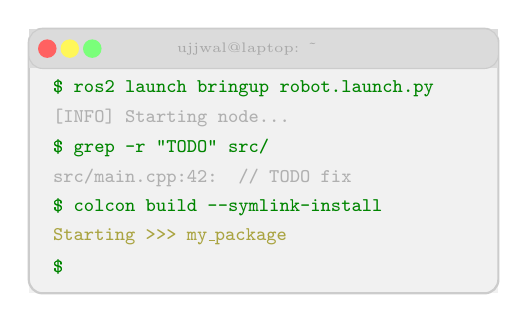
\begin{tikzpicture}[scale=0.84]
          \fill[gray!11] (0,0) rectangle (7.1,4.0);
          \draw[gray!40, rounded corners=5pt, thick] (0,0) rectangle (7.1,4.0);
          \fill[gray!28] (0,3.40) rectangle (7.1,4.0);
          \draw[gray!40, rounded corners=5pt] (0,3.40) rectangle (7.1,4.0);
          \fill[red!62]    (0.28,3.70) circle (0.14cm);
          \fill[yellow!65] (0.62,3.70) circle (0.14cm);
          \fill[green!52]  (0.96,3.70) circle (0.14cm);
          \node[font=\tiny, gray!68] at (3.30,3.70)
            {ujjwal@laptop: \textasciitilde};
          \node[font=\ttfamily\scriptsize, anchor=west, green!52!black]
            at (0.22,3.10) {\$ ros2 launch bringup robot.launch.py};
          \node[font=\ttfamily\scriptsize, anchor=west, gray!62]
            at (0.22,2.65) {[INFO] Starting node...};
          \node[font=\ttfamily\scriptsize, anchor=west, green!52!black]
            at (0.22,2.20) {\$ grep -r "TODO" src/};
          \node[font=\ttfamily\scriptsize, anchor=west, gray!62]
            at (0.22,1.75) {src/main.cpp:42: // TODO fix};
          \node[font=\ttfamily\scriptsize, anchor=west, green!52!black]
            at (0.22,1.30) {\$ colcon build --symlink-install};
          \node[font=\ttfamily\scriptsize, anchor=west, yellow!62!black]
            at (0.22,0.85) {Starting >>> my\_package};
          \node[font=\ttfamily\scriptsize, anchor=west, green!52!black]
            at (0.22,0.40) {\$};
        \end{tikzpicture}
      \end{center}
  \end{columns}
\end{frame}

\begin{frame}{Anatomy of the Prompt}
  \begin{center}
    {\ttfamily\large
      ujjwal\alert{@}laptop\alert{:}\textasciitilde/ros2\_ws\alert{\$}}
  \end{center}
  \vspace{0.6em}
  \begin{columns}
    \column{.25\textwidth}
      \begin{block}{\texttt{ujjwal}}
        \centering Username
      \end{block}
    \column{.25\textwidth}
      \begin{block}{\texttt{laptop}}
        \centering Hostname
      \end{block}
    \column{.25\textwidth}
      \begin{exampleblock}{\texttt{\textasciitilde/ros2\_ws}}
        \centering Current folder
      \end{exampleblock}
    \column{.25\textwidth}
      \begin{alertblock}{\texttt{\$}}
        \centering Prompt
      \end{alertblock}
  \end{columns}
  \vspace{0.5em}
  \begin{columns}
    \column{.5\textwidth}
      \begin{block}{\texttt{\$} -- regular user}
        Normal everyday work.
      \end{block}
    \column{.5\textwidth}
      \begin{alertblock}{\texttt{\#} -- root (superuser)}
        Never run as root for everyday tasks!
      \end{alertblock}
  \end{columns}
\end{frame}

\begin{frame}{Command Structure}
  \begin{center}
    {\ttfamily\large \alert{command}~[-options]~[parameters]}
  \end{center}
  \vspace{0.4em}
  \begin{columns}
    \column{.33\textwidth}
      \begin{block}{\texttt{command}}
        The program to run.
        If it is in \texttt{\$PATH},
        just type its name.
      \end{block}
    \column{.33\textwidth}
      \begin{exampleblock}{\texttt{[-options]}}
        Flags that change behaviour.\\[0.2em]
        Short: \texttt{-l}\\
        Long: \texttt{--long}\\
        Combined: \texttt{-la}
      \end{exampleblock}
    \column{.33\textwidth}
      \begin{block}{\texttt{[parameters]}}
        What to act on:
        files, folders,
        text strings \ldots
      \end{block}
  \end{columns}
  \vspace{0.4em}
  \begin{table}
    \begin{tabularx}{\textwidth}{lllX}
      \textbf{Command} & \textbf{Options} & \textbf{Parameter}
        & \textbf{What it does} \\
      \toprule
      \texttt{ls}   & \texttt{-la} & \texttt{\textasciitilde}
        & list all files in home (long format) \\
      \texttt{cp}   & \texttt{-r}  & \texttt{src/ dst/}
        & copy folder recursively \\
      \texttt{grep} & \texttt{-r}  & \texttt{"TODO" src/}
        & search recursively in src/ \\
      \bottomrule
    \end{tabularx}
  \end{table}
\end{frame}

\begin{frame}{Getting Help}
  \begin{columns}
    \column{.5\textwidth}
      \begin{block}{\texttt{man <command>}}
        Full manual page.\\[0.3em]
        \begin{itemize}
          \item Arrow keys to scroll
          \item \texttt{/} to search
          \item \texttt{q} to quit
        \end{itemize}
        \vspace{0.2em}
        \texttt{man ls} \quad \texttt{man grep} \quad \texttt{man cp}
      \end{block}
    \column{.5\textwidth}
      \begin{block}{\texttt{command --help} / \texttt{-h}}
        Short summary of options.
        Usually fits one screen.\\[0.2em]
        Long options use \texttt{--} (two dashes):\\
        \texttt{ls --help} \quad \texttt{git --version}\\[0.2em]
        Short options use \texttt{-} (one dash):\\
        \texttt{ls -h} \quad \texttt{colcon -h}
      \end{block}
  \end{columns}
  \vspace{0.5em}
  \begin{exampleblock}{Bonus: \texttt{tldr} (install separately)}
    \texttt{sudo apt install tldr} \quad then \quad \texttt{tldr ls}\\
    Shows practical examples instead of full documentation.
    Great for quick lookups.
  \end{exampleblock}
\end{frame}

\begin{frame}{Tab Completion}
  \framesubtitle{The most useful shortcut you will learn today}
  \begin{columns}
    \column{.44\textwidth}
      \begin{center}
        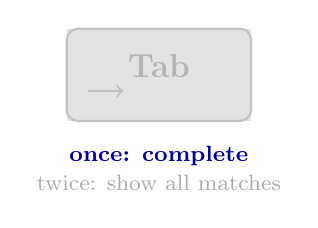
\begin{tikzpicture}[scale=0.90]
          \fill[gray!22] (0,0) rectangle (2.6,1.30);
          \draw[gray!48, rounded corners=4pt, thick]
            (0,0) rectangle (2.6,1.30);
          \node[font=\large\bfseries, gray!58] at (1.30,0.78) {Tab};
          \draw[->, thick, gray!48] (0.30,0.42) -- (0.80,0.42);
          % \node[font=\tiny, gray!55] at (1.30,0.22) {above Caps Lock};
          \node[font=\footnotesize\bfseries, blue!65!black]
            at (1.30,-0.50) {once: complete};
          \node[font=\footnotesize, gray!65]
            at (1.30,-0.88) {twice: show all matches};
        \end{tikzpicture}
      \end{center}
      \begin{exampleblock}{Tab completes}
        \begin{itemize}
          \item File and folder names
          \item Command names
          \item ROS2 topic and node names
        \end{itemize}
      \end{exampleblock}
    \column{.56\textwidth}
      \begin{block}{Example}
        Type \texttt{cd Do} then Tab Tab:\\[0.2em]
        \texttt{Documents/} \quad \texttt{Downloads/}\\[0.3em]
        Type \texttt{cd Dow} then Tab:\\[0.2em]
        $\rightarrow$ completes to \texttt{cd Downloads/}
      \end{block}
      \begin{alertblock}{Use Tab constantly}
    It prevents typos and instantly tells you if a file or command does not exist.
  \end{alertblock}
  \end{columns}
  
\end{frame}

% ====================================================================
\section{Files and Directories}
\subsection{Navigation}
% ====================================================================

\begin{frame}[fragile]{Navigation: pwd and ls}
  \begin{columns}
    \column{.38\textwidth}
      \begin{block}{\texttt{pwd}}
        Print Working Directory.\\
        ``Where am I right now?''
      \end{block}
      \vspace{0.4em}
      \begin{block}{\texttt{ls [options] [path]}}
        List directory contents.\\[0.3em]
        \texttt{-l} \quad long format\\
        \texttt{-a} \quad show hidden files\\
        \texttt{-h} \quad human-readable sizes\\
        \texttt{-la} \quad combine flags
      \end{block}
    \column{.62\textwidth}
        \begin{lstlisting}[language=bash]
$ pwd
/home/ujjwal/ros2_ws

$ ls
src  build  install  log

$ ls -la ~/ros2_ws
drwxr-xr-x 4 ujjwal ujjwal  80 Sep 10 ros2_ws
drwxr-xr-x 8 ujjwal ujjwal 160 Sep 10 src
        \end{lstlisting}
  \end{columns}
\end{frame}

\begin{frame}[fragile]{Navigation: cd}
  \framesubtitle{Change Directory}
  \begin{columns}
    \column{.40\textwidth}
      \footnotesize
      \begin{tabularx}{\columnwidth}{lX}
        \textbf{Path} & \textbf{Meaning} \\
        \toprule
        \texttt{/}  & Root of the filesystem \\
        \texttt{\textasciitilde} & Your home folder \\
        \texttt{.}  & Current directory \\
        \texttt{..} & Parent directory \\
        \texttt{-}  & Previous directory \\
        \bottomrule
      \end{tabularx}
      \vspace{0.5em}
      \normalsize
      \begin{exampleblock}{Tip}
        \texttt{cd -} jumps back to your
        last directory. Great for switching
        between two folders quickly.
      \end{exampleblock}
    \column{.60\textwidth}
        \begin{lstlisting}[language=bash]
$ cd ~/ros2_ws      # go to ros2_ws in home
$ cd src            # relative: go into src/
$ cd ..             # go up one level
$ cd ../..          # go up two levels
$ cd -              # go back to previous dir
$ cd                # go home (no argument)
        \end{lstlisting}
  \end{columns}
\end{frame}

\subsection{File Operations}

\begin{frame}[fragile]{Creating Directories: mkdir}
  \begin{columns}
    \column{.40\textwidth}
      \begin{block}{\texttt{mkdir [-p] <name>}}
        Create a new directory.\\[0.3em]
        \texttt{-p} also creates all missing
        parent directories. Never fails if the
        folder already exists.
      \end{block}
      \vspace{0.4em}
      \begin{exampleblock}{ROS2 workspace}
        \texttt{mkdir -p \textasciitilde/ros2\_ws/src}\\[0.2em]
        Creates both \texttt{ros2\_ws/} and \texttt{src/}
        in one command.
      \end{exampleblock}
    \column{.60\textwidth}
        \begin{lstlisting}[language=bash]
# Create a single folder
$ mkdir my_package

# Create nested folders (-p = parents too)
$ mkdir -p ~/ros2_ws/src/my_package/include

# Verify
$ ls ~/ros2_ws/src/
my_package
        \end{lstlisting}
  \end{columns}
\end{frame}

\begin{frame}[fragile]{Copying and Moving}
  \begin{columns}
    \column{.40\textwidth}
      \begin{block}{\texttt{cp [-r] <src> <dst>}}
        Copy a file or folder.\\
        \texttt{-r} required for directories.
      \end{block}
      \vspace{0.4em}
      \begin{block}{\texttt{mv <src> <dst>}}
        Move \textbf{or rename} a file.\\
        Works on directories too.\\
        No \texttt{-r} flag needed.
      \end{block}
    \column{.60\textwidth}
        \begin{lstlisting}[language=bash]
# Copy a file
$ cp main.cpp backup.cpp

# Copy an entire folder
$ cp -r src/ src_backup/

# Rename a file
$ mv old_name.cpp new_name.cpp

# Move file to another directory
$ mv robot.cpp ~/ros2_ws/src/my_pkg/

# Move multiple files at once
$ mv *.cpp ~/ros2_ws/src/my_pkg/
        \end{lstlisting}
  \end{columns}
\end{frame}

\begin{frame}[fragile]{Removing Files: rm}
  \begin{columns}
    \column{.40\textwidth}
      \begin{block}{\texttt{rm [-r] <name>}}
        Remove a file or folder.\\
        \texttt{-r} = recursive (entire folder).\\
        \texttt{-f} = force, no confirmation.
      \end{block}
      \vspace{0.3em}
      \begin{alertblock}{No recycle bin!}
        Files deleted with \texttt{rm} are
        \textbf{gone immediately}.
        No undo. No trash.\\[0.3em]
        Always \texttt{ls} first to see
        what you are about to delete.
      \end{alertblock}
    \column{.60\textwidth}
        \begin{lstlisting}[language=bash]
# Delete a file
$ rm old_file.cpp

# Delete a folder and all its contents
$ rm -r old_folder/

# Force delete, no prompts
$ rm -rf old_folder/

# Safe workflow: check first!
$ ls *.o        # see what will be deleted
$ rm *.o        # then delete
        \end{lstlisting}
  \end{columns}
\end{frame}

\begin{frame}[fragile]{Wildcards}
  \begin{columns}
    \column{.40\textwidth}
      \footnotesize
      \begin{tabularx}{\columnwidth}{lX}
        \textbf{Pattern} & \textbf{Matches} \\
        \toprule
        \texttt{*}         & Any set of chars \\
        \texttt{?}         & Exactly one char \\
        \texttt{[a-f]}     & Char in range a to f \\
        \texttt{[\^{}abc]} & Char NOT in abc \\
        \bottomrule
      \end{tabularx}
      \vspace{0.5em}
      \normalsize
      \begin{exampleblock}{Safe delete workflow}
        Step 1: \texttt{ls *.o}\\
        \hspace*{1em}(check what matches)\\[0.2em]
        Step 2: \texttt{rm *.o}\\
        \hspace*{1em}(then delete safely)
      \end{exampleblock}
    \column{.60\textwidth}
        \begin{lstlisting}[language=bash]
$ ls *.cpp          # all .cpp files
main.cpp  robot.cpp  utils.cpp

$ ls v0?.pdf        # v01.pdf, v02.pdf, ...
v01.pdf  v02.pdf

$ ls [uv]01*        # u01.tex, v01.pdf, ...
u01.tex  v01.pdf  v01.tex

$ rm *.o            # delete all object files
$ cp *.h include/   # copy all headers
        \end{lstlisting}
  \end{columns}
\end{frame}

% ====================================================================
\section{Input, Output, and Pipes}
\subsection{Standard I/O}
% ====================================================================

\begin{frame}{Standard I/O Channels}
  \framesubtitle{Every program has three default channels}
  \begin{center}
    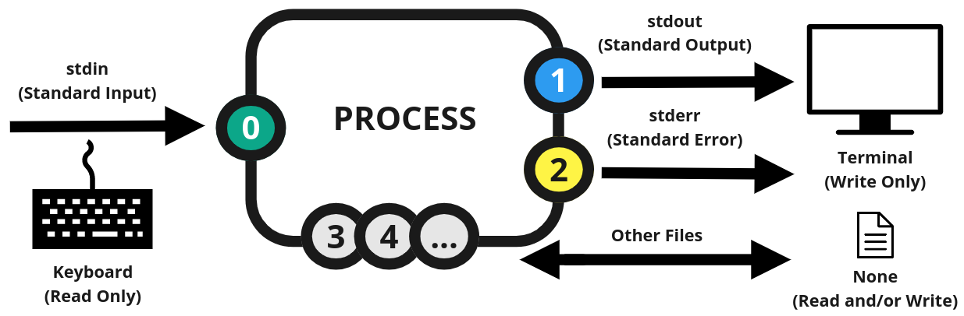
\includegraphics[width=0.80\textwidth, keepaspectratio]{stdio_diagram.png}
  \end{center}
  \vspace{0.3em}
  \begin{columns}
    \column{.33\textwidth}
      \begin{block}{\texttt{stdin} -- channel 0}
        \centering Keyboard by default\\
        \texttt{std::cin}
      \end{block}
    \column{.33\textwidth}
      \begin{block}{\texttt{stdout} -- channel 1}
        \centering Normal output\\
        \texttt{std::cout}
      \end{block}
    \column{.33\textwidth}
      \begin{alertblock}{\texttt{stderr} -- channel 2}
        \centering Error messages\\
        \texttt{std::cerr}
      \end{alertblock}
  \end{columns}
\end{frame}

\begin{frame}[fragile]{Redirecting I/O}
  \begin{columns}
    \column{.38\textwidth}
      \small
      \begin{itemize}
        \item \alert{\texttt{>}} \quad redirect, overwrite
        \item \alert{\texttt{>{}>}} \quad redirect, append
        \item \alert{\texttt{<}} \quad feed file as stdin
        \item \alert{\texttt{2>\&1}} \quad merge stderr into stdout
        \item \texttt{/dev/null} -- discard all output
      \end{itemize}
      
    \column{.62\textwidth}
        \begin{lstlisting}[language=bash,basicstyle=\ttfamily\scriptsize]
$ program 1> output.txt   # stdout to file
$ program 2> errors.txt   # stderr to file
$ program 1> out.txt 2> err.txt  # separate

$ program 1> all.txt 2>&1 # both to same file
$ program < input.txt     # feed file as stdin

# Append without overwriting
$ echo "hello" >> log.txt

# Discard all output
$ program > /dev/null 2>&1
        \end{lstlisting}
  \end{columns}
  \begin{exampleblock}{ROS2 log}
        Save all launch output:\\
        \texttt{ros2 launch bringup robot.launch.py}\\
        \texttt{1>log.txt 2>\&1}
      \end{exampleblock}
\end{frame}

\subsection{Pipes and Searching}

\begin{frame}[fragile]{Pipes and Command Chaining}
  \begin{columns}
    \column{.38\textwidth}
      \begin{block}{\texttt{cmd1 | cmd2}}
        stdout of \texttt{cmd1} becomes stdin
        of \texttt{cmd2}. Chain as many as needed.
      \end{block}
      \vspace{0.4em}
      \footnotesize
      \begin{tabularx}{\columnwidth}{lX}
        \textbf{Op} & \textbf{Behaviour} \\
        \toprule
        \texttt{;}    & run always \\
        \texttt{\&\&} & run if prev OK \\
        \texttt{||}   & run if FAILED \\
        \bottomrule
      \end{tabularx}
      \normalsize
    \column{.62\textwidth}
        \begin{lstlisting}[language=bash]
# Pipe: stdout of left -> stdin of right
$ ls | grep ".cpp"

# Chain multiple programs
$ cat log.txt | grep ERROR | sort | uniq

# ; runs next regardless of success
$ mkdir build ; cd build

# && runs next only if previous succeeded
$ mkdir build && cd build && cmake ..

# || runs next only if previous FAILED
$ test -f config.yaml || echo "Missing!"
        \end{lstlisting}
  \end{columns}
\end{frame}

\begin{frame}[fragile]{Viewing and Searching Files}
  \begin{columns}
    \column{.36\textwidth}
      \begin{block}{View file contents}
        \begin{itemize}
          \item \texttt{cat} -- print whole file
          \item \texttt{less} -- scroll (\texttt{q} to quit)
          \item \texttt{head -n N} -- first N lines
          \item \texttt{tail -n N} -- last N lines
          \item \texttt{tail -f} -- follow live
        \end{itemize}
      \end{block}
      \vspace{0.3em}
      \begin{block}{Search}
        \begin{itemize}
          \item \texttt{grep} -- search inside files
          \item \texttt{find} -- find files by name
        \end{itemize}
      \end{block}
    \column{.64\textwidth}
        \begin{lstlisting}[language=bash]
$ cat CMakeLists.txt     # print whole file
$ less build.log         # scroll (q to quit)
$ head -n 20 output.txt  # first 20 lines
$ tail -n 20 output.txt  # last 20 lines
$ tail -f output.txt     # follow live output

$ grep "TODO" src/main.cpp
$ grep -r "ros::init" src/  # recursive

$ find ~/ros2_ws -name "*.cpp"
$ find . -name "CMakeLists.txt"
        \end{lstlisting}
  \end{columns}
\end{frame}

% ====================================================================
\section{System Management}
\subsection{History and Processes}
% ====================================================================

\begin{frame}[fragile, shrink=5]{Command History}
  \begin{columns}
    \column{.44\textwidth}
      \footnotesize
      \begin{tabularx}{\columnwidth}{lX}
        \textbf{Key / Command} & \textbf{Action} \\
        \toprule
        $\uparrow$ / $\downarrow$ & scroll history \\
        Ctrl + R         & search history \\
        \texttt{history} & show full list \\
        \texttt{!N}      & run command N \\
        \texttt{!!}      & repeat last \\
        \texttt{sudo !!} & with sudo \\
        \bottomrule
      \end{tabularx}
      \normalsize
    \column{.56\textwidth}
        \begin{lstlisting}[language=bash]
$ history
  421  cd ~/ros2_ws
  422  colcon build
  423  ros2 run my_pkg my_node

$ !423       # re-run command 423
$ !!         # re-run last command
$ sudo !!    # re-run last with sudo
        \end{lstlisting}
      \vspace{0.3em}
      \begin{exampleblock}{Ctrl + R search}
        Press Ctrl+R, start typing.
        The shell searches backwards through history.
        Press Enter to run the found command.
      \end{exampleblock}
  \end{columns}
\end{frame}

\begin{frame}[fragile, shrink=5]{Managing Processes}
  \begin{columns}
    \column{.44\textwidth}
      \footnotesize
      \begin{tabularx}{\columnwidth}{lX}
        \textbf{Key / Command} & \textbf{Action} \\
        \toprule
        Ctrl + C         & cancel \\
        Ctrl + Z         & suspend \\
        \texttt{bg}      & resume in bg \\
        \texttt{fg}      & bring to fg \\
        \texttt{cmd \&}  & start in bg \\
        \texttt{kill -9} & force kill \\
        \texttt{killall} & kill by name \\
        \texttt{htop}    & visual viewer \\
        \bottomrule
      \end{tabularx}
      \normalsize
    \column{.56\textwidth}
        \begin{lstlisting}[language=bash]
# Run in the background
$ ros2 run my_pkg my_node &
[1] 12345

# Find the process
$ ps aux | grep my_node

# Kill by PID
$ kill -9 12345

# Kill by name
$ killall rviz2
        \end{lstlisting}
      \vspace{0.3em}
      \begin{exampleblock}{\texttt{htop}}
        Run \texttt{htop} for a live process manager.
        Arrow keys to navigate,
        F9 to kill, q to quit.
      \end{exampleblock}
  \end{columns}
\end{frame}

\subsection{Installing Software}

\begin{frame}[fragile]{Installing Software with APT}
  \begin{columns}
    \column{.38\textwidth}
      \small
      \begin{block}{APT -- Advanced Package Tool}
        Ubuntu's official package manager.
        Downloads from trusted \alert{repositories}.
        Always run \texttt{apt update} first.
      \end{block}
      \vspace{0.3em}
      \begin{exampleblock}{ROS2 packages}
        \texttt{sudo apt install}\\
        \texttt{ros-humble-rviz2}\\[0.2em]
        Libraries: prefix \texttt{lib},
        suffix \texttt{-dev}
      \end{exampleblock}
    \column{.62\textwidth}
        \begin{lstlisting}[language=bash,basicstyle=\ttfamily\scriptsize]
$ sudo apt update              # refresh
$ sudo apt upgrade             # upgrade all

$ sudo apt install vim         # install
$ sudo apt install libopencv-dev

$ apt search opencv            # search

$ sudo apt remove vim          # remove
        \end{lstlisting}
  \end{columns}
\end{frame}

% ====================================================================
\section{Terminal Editors}
\subsection{nano}
% ====================================================================

\begin{frame}{Why Terminal Editors?}
  \begin{columns}
    \column{.5\textwidth}
      \begin{alertblock}{When you will need one}
        \begin{itemize}
          \item SSH into a robot -- no GUI available
          \item Quick edit of a config or launch file
          \item GUI broke after a bad update
          \item Inside Docker or Distrobox
          \item Editing a file owned by root
        \end{itemize}
      \end{alertblock}
    \column{.5\textwidth}
      \begin{block}{Two editors to learn}
        \begin{itemize}
          \item \textbf{nano} -- beginner-friendly.
                Controls shown on screen.
                No modes. Works immediately.
          \vspace{0.4em}
          \item \textbf{vim} -- fast, powerful.
                Available on every Linux system.
                Learning curve, but worth it.
        \end{itemize}
      \end{block}
      \vspace{0.4em}
      \begin{exampleblock}{Both already installed}
        No setup needed on Ubuntu.
      \end{exampleblock}
  \end{columns}
\end{frame}

\begin{frame}[fragile]{nano -- Basics}
  \framesubtitle{The beginner-friendly terminal editor}
  \begin{columns}
    \column{.44\textwidth}
        \begin{lstlisting}[language=bash,basicstyle=\ttfamily\scriptsize]
$ nano ~/.bashrc       # open
$ nano new_script.sh   # new file
$ nano -l config.yaml  # line #s
        \end{lstlisting}
      \vspace{0.2em}
      \small
      \begin{itemize}
        \item Just type -- no modes to switch
        \item Arrow keys to move
        \item \alert{\textasciicircum} means \alert{Ctrl}
        \item All shortcuts shown \alert{at the bottom}
      \end{itemize}
      \vspace{0.15em}
      \begin{exampleblock}{Beginner workflow}
        Open $\rightarrow$ edit $\rightarrow$ save $\rightarrow$ exit
      \end{exampleblock}
    \column{.56\textwidth}
      \begin{center}
        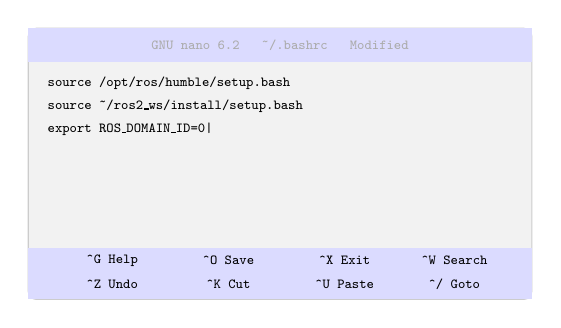
\begin{tikzpicture}[scale=0.82]
          \fill[gray!10] (0,0) rectangle (7.8,4.2);
          \draw[gray!40, rounded corners=3pt] (0,0) rectangle (7.8,4.2);
          \fill[blue!14] (0,3.68) rectangle (7.8,4.2);
          \node[font=\ttfamily\tiny, gray!65] at (3.90,3.94)
            {GNU nano 6.2 \quad \textasciitilde/.bashrc \quad Modified};
          \node[font=\ttfamily\tiny, anchor=north west] at (0.15,3.60)
            {source /opt/ros/humble/setup.bash};
          \node[font=\ttfamily\tiny, anchor=north west] at (0.15,3.24)
            {source \textasciitilde/ros2\_ws/install/setup.bash};
          \node[font=\ttfamily\tiny, anchor=north west] at (0.15,2.88)
            {export ROS\_DOMAIN\_ID=0|};
          \fill[blue!14] (0,0) rectangle (7.8,0.80);
          \node[font=\ttfamily\tiny] at (1.30,0.60)
            {\textasciicircum{}G Help};
          \node[font=\ttfamily\tiny] at (3.10,0.60)
            {\textasciicircum{}O Save};
          \node[font=\ttfamily\tiny] at (4.90,0.60)
            {\textasciicircum{}X Exit};
          \node[font=\ttfamily\tiny] at (6.60,0.60)
            {\textasciicircum{}W Search};
          \node[font=\ttfamily\tiny] at (1.30,0.24)
            {\textasciicircum{}Z Undo};
          \node[font=\ttfamily\tiny] at (3.10,0.24)
            {\textasciicircum{}K Cut};
          \node[font=\ttfamily\tiny] at (4.90,0.24)
            {\textasciicircum{}U Paste};
          \node[font=\ttfamily\tiny] at (6.60,0.24)
            {\textasciicircum{}/ Goto};
        \end{tikzpicture}
      \end{center}
  \end{columns}
\end{frame}

\begin{frame}{nano -- Key Reference}
  \begin{table}
    \begin{tabularx}{\textwidth}{llX}
      \textbf{Shortcut} & \textbf{Keys} & \textbf{Action} \\
      \toprule
      \texttt{\textasciicircum{}O} & Ctrl + O
        & \textbf{Save} the file (press Enter to confirm) \\
      \texttt{\textasciicircum{}X} & Ctrl + X
        & \textbf{Exit} (asks to save if unsaved changes exist) \\
      \texttt{\textasciicircum{}W} & Ctrl + W
        & \textbf{Search} -- type term, press Enter \\
      \texttt{\textasciicircum{}K} & Ctrl + K
        & \textbf{Cut} the current line \\
      \texttt{\textasciicircum{}U} & Ctrl + U
        & \textbf{Paste} the cut line \\
      \texttt{\textasciicircum{}Z} & Ctrl + Z
        & \textbf{Undo} last change \\
      \texttt{\textasciicircum{}/} & Ctrl + /
        & \textbf{Go to line} number \\
      \texttt{\textasciicircum{}G} & Ctrl + G
        & \textbf{Help} -- full shortcut reference \\
      \bottomrule
    \end{tabularx}
  \end{table}
  \vspace{0.3em}
  \begin{exampleblock}{\textasciicircum{} means Ctrl}
    \texttt{\textasciicircum{}O} = hold Ctrl and press O.
    You do not type the caret symbol.
  \end{exampleblock}
\end{frame}

\subsection{vim}

\begin{frame}{vim -- Introduction}
  \framesubtitle{Vi IMproved -- the editor available on every Linux system}
  \begin{columns}
    \column{.5\textwidth}
      \begin{itemize}
        \item Pre-installed on virtually every Linux system
        \item Keyboard-only -- no mouse needed
        \item Extremely fast once the muscle memory is built
        \item \alert{Modal editor} -- the same key does
              different things in different modes
      \end{itemize}
      \begin{block}{Opening vim}
        \texttt{vim \textasciitilde/.bashrc}\\
        \texttt{vim new\_file.py}\\
        \texttt{vim src/main.cpp}
      \end{block}
    \column{.5\textwidth}
      \begin{alertblock}{Stuck inside vim?}
        Press \texttt{Esc}, then type \texttt{:q!},
        then press Enter.\\[0.3em]
        Exits \textbf{without saving}.
        The most Googled Linux question.
      \end{alertblock}
      \vspace{0.4em}
      \begin{exampleblock}{Built-in tutorial}
        Run \texttt{vimtutor} in the terminal
        for a 30-minute interactive guide.
        Strongly recommended.
      \end{exampleblock}
  \end{columns}
\end{frame}

\begin{frame}{vim -- Modes}
  \framesubtitle{Understanding modes is the key to using vim}
  \begin{columns}
    \column{.52\textwidth}
      \begin{center}
        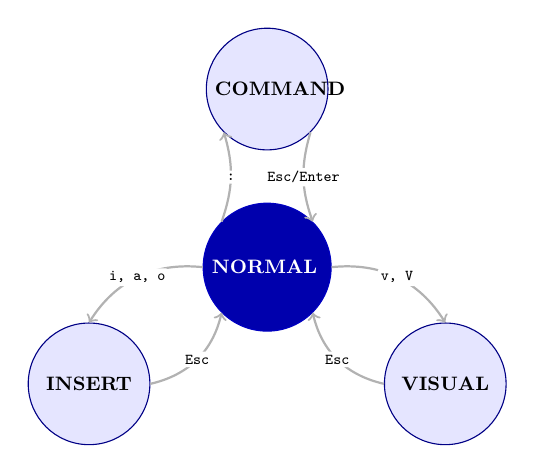
\begin{tikzpicture}[
          scale=0.78, transform shape,
          mode/.style={circle, draw=blue!52!black, fill=blue!10,
                       minimum size=1.90cm, font=\small\bfseries,
                       text centered, text width=1.70cm},
          home/.style={circle, draw=blue!76!black, fill=blue!68!black,
                       text=white, minimum size=2.00cm, font=\small\bfseries,
                       text width=1.80cm},
          arr/.style={->, thick, gray!60},
          lbl/.style={font=\scriptsize\ttfamily, text=black, fill=white,
                      inner sep=1.5pt, rounded corners=1pt}
        ]
          \node[home] (N) at (0,0)       {NORMAL};
          \node[mode] (I) at (-2.9,-1.9) {INSERT};
          \node[mode] (V) at  (2.9,-1.9) {VISUAL};
          \node[mode] (C) at  (0, 2.9)   {COMMAND};
          \draw[arr] (N.west) to[bend right=32]
            node[lbl, midway] {i, a, o} (I.north);
          \draw[arr] (I.east) to[bend right=32]
            node[lbl, midway] {Esc} (N.south west);
          \draw[arr] (N.east) to[bend left=32]
            node[lbl, midway] {v, V} (V.north);
          \draw[arr] (V.west) to[bend left=32]
            node[lbl, midway] {Esc} (N.south east);
          \draw[arr] (N.north west) to[bend right=18]
            node[lbl, midway] {:} (C.south west);
          \draw[arr] (C.south east) to[bend right=18]
            node[lbl, midway] {Esc/Enter} (N.north east);
        \end{tikzpicture}
      \end{center}
    \column{.48\textwidth}
      \small
      \begin{block}{NORMAL mode}
        Default. Navigate and run commands.
        Press \texttt{Esc} to always return here.
      \end{block}
      \vspace{0.15em}
      \begin{exampleblock}{INSERT mode}
        Type text. Enter: \texttt{i}, \texttt{a}, \texttt{o}.
      \end{exampleblock}
      \vspace{0.15em}
      \begin{block}{VISUAL mode}
        Select text. Enter: \texttt{v} or \texttt{V}.
      \end{block}
      \vspace{0.15em}
      \begin{alertblock}{COMMAND mode}
        Type after \texttt{:}. Save, quit, search/replace.
      \end{alertblock}
  \end{columns}
\end{frame}

\begin{frame}{vim -- Moving and Editing}
  \framesubtitle{All of these work in NORMAL mode}
  \begin{columns}
    \column{.5\textwidth}
      \begin{block}{Navigation}
        \begin{itemize}
          \item \texttt{h j k l} \quad left, down, up, right
          \item \texttt{w} \quad next word \quad \texttt{b} \quad back
          \item \texttt{0} \quad start of line \quad \texttt{\$} \quad end
          \item \texttt{gg} \quad top of file \quad \texttt{G} \quad bottom
          \item \texttt{:N} \quad jump to line N
        \end{itemize}
      \end{block}
    \column{.5\textwidth}
      \begin{block}{Editing}
        \begin{itemize}
          \item \texttt{dd} \quad delete (cut) current line
          \item \texttt{yy} \quad copy (yank) current line
          \item \texttt{p} \quad paste below cursor
          \item \texttt{u} \quad undo \quad Ctrl+R \quad redo
          \item \texttt{/word} \quad search for word
          \item \texttt{n} / \texttt{N} \quad next / previous match
        \end{itemize}
      \end{block}
  \end{columns}
\end{frame}

\begin{frame}{vim -- Saving and Quitting}
  \framesubtitle{Press : from NORMAL mode, type the command, press Enter}
  \begin{table}
    \begin{tabularx}{\textwidth}{llX}
      \textbf{Command} & \textbf{Entry} & \textbf{Action} \\
      \toprule
      \texttt{:w}             & Normal $\rightarrow$ \texttt{:}
        & Save (write to disk) \\
      \texttt{:q}             & Normal $\rightarrow$ \texttt{:}
        & Quit (fails if unsaved changes) \\
      \texttt{:wq}            & Normal $\rightarrow$ \texttt{:}
        & \textbf{Save and quit} \\
      \texttt{:q!}            & Normal $\rightarrow$ \texttt{:}
        & \textbf{Quit WITHOUT saving} (force) \\
      \texttt{:set number}    & Normal $\rightarrow$ \texttt{:}
        & Show line numbers \\
      \texttt{:\%s/old/new/g} & Normal $\rightarrow$ \texttt{:}
        & Replace all occurrences \\
      \bottomrule
    \end{tabularx}
  \end{table}
  \vspace{0.3em}
  \begin{columns}
    \column{.5\textwidth}
      \begin{exampleblock}{Insert mode entry}
        \texttt{i} before \quad \texttt{a} after \quad
        \texttt{o} new line below
      \end{exampleblock}
    \column{.5\textwidth}
      \begin{alertblock}{Golden rule}
        Always press \texttt{Esc} first to return
        to Normal mode before typing a command.
      \end{alertblock}
  \end{columns}
\end{frame}

% ====================================================================
\section{If Ubuntu 22.04 Does Not Work}
\subsection{Hardware Compatibility}
% ====================================================================

\begin{frame}{Why Ubuntu 22.04 May Struggle?}
  \framesubtitle{Default kernel 6.8 still struggles with newer Hardware}
  \begin{columns}
    \column{.5\textwidth}
      \begin{alertblock}{Common symptoms}
        \begin{itemize}
          \item Blank screen after installation
          \item System freezes when GPU switches
          \item Wi-Fi not detected at all
          \item Very poor battery or performance
        \end{itemize}
      \end{alertblock}
      \footnotesize
      \begin{exampleblock}{Quick try: HWE kernel}
        \texttt{sudo apt install linux-generic-hwe-22.04}\\[0.15em]
        Upgrades kernel to 6.8. Fixes some hardware --
        else see the three options below.
      \end{exampleblock}
    \column{.5\textwidth}
      \small
      \begin{block}{Commonly affected hardware}
        \begin{itemize}
          \item NVIDIA RTX 40 and 50 series
          \item AMD Ryzen 7000+ / Ryzen AI 300
          \item Intel BE200 Wi-Fi adapter
          \item Mediatek MT7922 Wi-Fi adapter
          \item Laptops with a MUX switch (hybrid GPU)
        \end{itemize}
      \end{block}
  \end{columns}
\end{frame}

\begin{frame}{Option 1: Ubuntu 24.04 LTS}
  \begin{columns}
    \column{.48\textwidth}
      \begin{block}{What changes}
        \begin{itemize}
          \item Ships kernel 6.8, \alert{HWE brings it to 7.0}
          \item Full support for RTX 40/50,
                Ryzen AI, new Wi-Fi chips
          \item ROS2 \alert{Jazzy} runs natively
        \end{itemize}
      \end{block}
      \vspace{0.3em}
      \begin{alertblock}{Trade-off}
        ROS2 \textbf{Humble} needs Docker on 24.04.
        Course materials target Humble.
      \end{alertblock}
    \column{.52\textwidth}
      \begin{exampleblock}{Steps}
        \begin{enumerate}
          \item Download Ubuntu 24.04 ISO from \url{ubuntu.com}
          \item Flash to USB (Balena Etcher or Rufus)
          \item Install alongside Windows (dual boot)
          \item Install ROS2 Humble via Docker
        \end{enumerate}
      \end{exampleblock}
      \vspace{0.4em}
      \begin{block}{Best for}
        Post-2022 hardware without a dedicated NVIDIA GPU.
      \end{block}
  \end{columns}
\end{frame}

\begin{frame}[fragile]{Option 2: Fedora + Distrobox}
  \begin{columns}
    \column{.5\textwidth}
      \begin{block}{What is Distrobox?}
        Runs any Linux distro as a \alert{container}
        inside your host OS. Shares your home folder,
        GPU, and hardware. Near-native performance.
      \end{block}
      \vspace{0.3em}
      \begin{itemize}
        \item Fedora ships with \alert{kernel 7.1+}
        \item Distrobox gives full Ubuntu 22.04 inside
        \item ROS2 Humble runs natively in the container
        \item Files and hardware work normally
      \end{itemize}
    \column{.5\textwidth}
        \begin{lstlisting}[language=bash]
# Install on Fedora
$ sudo dnf install distrobox podman

# Create Ubuntu 22.04 container
$ distrobox create -n ros-humble \
    -i ubuntu:22.04

# Enter the container
$ distrobox enter ros-humble

# Now inside Ubuntu 22.04
# Install ROS2 Humble normally
        \end{lstlisting}
    \begin{exampleblock}{Best for}
        All gaming laptops, especially AMD.
      \end{exampleblock}
  \end{columns}
\end{frame}

\begin{frame}{Option 3: NVIDIA Laptop -- dGPU Only Mode}
  \begin{columns}
    \column{.52\textwidth}
      \begin{block}{The problem}
        Modern NVIDIA laptops have \alert{hybrid graphics}:
        iGPU for battery life and dGPU for performance.
        The MUX switch between them causes kernel panics
        on Ubuntu 22.04.
      \end{block}
      \vspace{0.4em}
      \begin{exampleblock}{The fix -- in BIOS/UEFI}
        \begin{enumerate}
          \item Restart -- press Del / F2 / F12
          \item Advanced $\rightarrow$ Display $\rightarrow$ GPU Mode
          \item Set to \alert{dGPU Only} or Discrete GPU
          \item Save and exit
        \end{enumerate}
      \end{exampleblock}
    \column{.48\textwidth}
      \begin{alertblock}{Consequences}
        Higher power use -- keep power brick plugged in.
        Battery life drops noticeably.
      \end{alertblock}
      \vspace{0.4em}
      \begin{block}{Benefit}
        No driver workarounds needed.
        Ubuntu 22.04 and ROS2 Humble work cleanly.
      \end{block}
      \vspace{0.4em}
      \begin{exampleblock}{Best for}
        ASUS ROG, MSI, Razer, Lenovo Legion (NVIDIA)
      \end{exampleblock}
  \end{columns}
\end{frame}

\begin{frame}[shrink=5]{Which Option Should I Choose?}
  \small
  \begin{table}
    \begin{tabularx}{\textwidth}{lXXXX}
      & \textbf{Ubuntu 22.04}
      & \textbf{Ubuntu 24.04}
      & \textbf{Fedora + Distrobox}
      & \textbf{dGPU Only} \\
      \toprule
      \textbf{Kernel}
        & 5.15 (HWE: 6.8) & 7.0 (HWE) & 7.1+ & 5.15 (HWE: 6.8) \\
      \textbf{ROS2 Humble}
        & Native & Via Docker & In container & Native \\
      \textbf{Difficulty}
        & Easy & Easy & Medium & Easy \\
      \textbf{Overhead}
        & None & None & Minimal & High power \\
      \textbf{Best for}
        & Works already & Mid hardware & Gaming laptops & NVIDIA laptops \\
      \bottomrule
    \end{tabularx}
  \end{table}
  \vspace{0.4em}
  \begin{block}{Quick decision guide}
    Ubuntu 22.04 installs fine $\rightarrow$ use it.\\
    NVIDIA gaming laptop $\rightarrow$ try dGPU Only first (easiest).\\
    AMD gaming laptop $\rightarrow$ Fedora + Distrobox.\\
    Nothing works $\rightarrow$ Ubuntu 24.04 + Docker.
  \end{block}
\end{frame}

\begin{frame}{Thank You}
  \begin{center}
    \vspace{0.5em}
    {\Large\textbf{Questions?}}\\[1.2em]
    {\large Introduction to Linux}\\[0.3em]
    {\normalsize Foundation Course -- Winter Semester 2026}\\[0.3em]
    {\normalsize Ujjwal Patil \quad H-BRS}\\[1.2em]
    \begin{block}{Further reading and practice}
      \texttt{man bash} \quad
      \texttt{vimtutor} \quad
      \url{https://ubuntu.com/tutorials}
    \end{block}
  \end{center}
\end{frame}

\end{document}
